
The proposed resource will distribute behavioural and electrophysiological data
from our foraging experiments and machine learning methods to simulate and analyse
these data. We will initially contribute to the resource machine learning
methods that we have used for the analysis of our foraging data. We will later
invite method contributions from external method developers. To motivate these
contributions we will organise foraging data simulation and data analysis
competitions.

\subsubsection{Distribution of long-duration and naturalistic foraging data}

We will distribute in the \href{https://dandiarchive.org/}{DANDI} archive data
and metadata generated in our foraging experiments.

The data will include
video recordings from all cameras,
foraging wheels positions from all patches,
pellet delivery times from all patches,
mice weights recorded at the nest and
ultrasound recordings of mice vocalisations.

The metadata will include
subject information (birth data, sex and genetic strain) and
experiment information (start date, duration and type -- single or multiple
mice).

We will also provide Python routines to access specific data and meta data
items from the raw
files\footnote{\url{https://github.com/SainsburyWellcomeCentre/aeon_mecha}}.

The data generated by our experiments is very large. Storing one hour of
electrophysiological recordings requires xx gigabytes and one hour of video
recordings requires yy gigabytes. For this reason we will initially only share
publicly in the \href{https://dandiarchive.org/}{DANDI} archive a small number
of experimental sessions.
%
Investigating alternative methods to share the large amounts of data generated
by our experiments is a research item proposed for this resource
(Section~\ref{sec:research}).

\subsubsection{Methods for data analysis}

Below we describe a few methods that we have used, or plan to use, to
control/characterize our foraging data. We may or may not use all of these
methods, or we may use other methods not listed there. It is difficult to
anticipate the challenges that we might encounter when processing our
long-duration, multi-modal and complex datasets, specially when adding to the
analysis electrophysiological recordings. Yet we are confident that we will
excel on this processing, as we are a team with unique experience to do so
(Section~\ref{sec:teamCapability}).

\paragraph{Linear dynamical systems models}

Linear dynamical systems (LDS) models are used to characterise time-varying
observations as a function of hidden (i.e., latent) continuous state variables
that vary over time. It assumes that both state and observations are Gaussian
random vectors. The Kalman filter algorithm can be used to infer the
probability distribution of the state given observations. More information
about LDS models can be found in \citep[][part I]{durbinAndKoopman12}. They can
be used to model behavioural and neural data.

We have developed an implementation of LDS
models\footnote{\url{https://github.com/joacorapela/lds\_python}} and used it to infer denoised
positions, velocities and accelerations of foraging mice from noisy and
incomplete position measurements
\href{https://joacorapela.github.io/lds\_python/auto\_examples/tracking/plotFilterFWGMouseTrajectoryManualVsLearnedParams.html}{offline}
and
\href{https://bonsai-rx.org/machinelearning/examples/examples/LinearDynamicalSystems/Kinematics/ForagingMouse/README.html}{online}
with Bonsai.
%
We have also used this implementation to characterise electrophysiological recordings in mice.

\paragraph{Nonlinear and non-Gaussian dynamical systems models}

LDS models are very versatile and can be used to model a wide range of
time-series observations. However, there are cases where this model does not
apply and nonlinear and non-Gaussians extensions are needed, like extended
Kalman filter, the unscented Kalman filter and the particle
filter~\citep[][part II]{durbinAndKoopman12}.

We have created the Poisson Linear Dynamical System (PLDS) model to characterise count
observations~\citep{mackeEtAl15} and distributed a Matlab
implementation\footnote{\url{https://bitbucket.org/mackelab/pop\_spike\_dyn}}.
This is an offline implementation, and we have not yet produced an online one.
We have neither use PLDS to model behavioural or neural foraging data.

\paragraph{Gaussian processes models}

Gaussian process factor analysis (GPFA) models~\citep{yuEtAl09} are similar to
LDS ones in that the probability distribution of observation is a function of
latent variable. However, differently from LDS, where latent variables have
linear dynamics, in GPFA models latent variables are samples from a Gaussian
process and have nonlinear dynamics. We contributed to the development of a
Matlab implementation of
GPFA\footnote{\url{https://users.ece.cmu.edu/~byronyu/software.shtml}}.

GPFA is used to characterise neural activity. It requires binning of spikes
into spikes counts and assumes that spike counts follow a Gaussian
distribution. We have recently introduced sparse variational Gaussian process
factor analysis~\citep[svGPFA,][]{dunckerAndSahani18} that uses point process observations
and does not require to bin spikes times and developed a Python implementation
of it\footnote{\url{https://github.com/joacorapela/svGPFA}}.

We have not yet attempted online versions of these algorithms.

\paragraph{Hidden Markov models}

The hidden Markov model (HMM) is a latent variable model similar to the LDS
model, but where the hidden states are discrete~\citep[][Chapter 13]{bishop06}. It is
used to assign discrete labels to time series observations.

We have developed an offline
implementation\footnote{\url{https://github.com/joacorapela/hiddenMarkovModels}}
of the HMM, used it to find repeatable states in epileptic seizures of human
subjects, from Utah array recordings of their neural
activity~\citep{rapelaAndTodorov19-epilepsy-hmm}. We have also used the HMM to
infer mouse foraging states from kinematic inferences from the LDS model. We
are currently building an online implementation of the HMM in Bonsai.

\paragraph{Switching linear dynamical systems models}

A switching linear dynamical system (SLDS) model is a hybrid/nonlinear system which
consists of several linear subsystems and a switching rule that decides which
of the subsystems is active at each moment in time \citep[Section
18.6]{murphy12}.

Over long periods of time the behaviour and neural activity of mice may
alternate between different states, where each state can be well modelled by a
linear dynamical system. Long-duration behavioural and neural time series could
be well modelled by SLDS models.

We have no yet used SLDS models to characterise our foraging data.

\paragraph{Recognition parameterised models}

\paragraph{Generalised linear models}

Generalised linear models (GLMs) are regression models for observations with diverse
noise distributions (i.e., noise distributions in the exponential family). For
example, they can be used to estimate a linear regression model with spike
count as the observation variable.

We have used a Gaussian GLM (i.e., a standard linear regression model) to
study how different regressors (e.g., average speed or acceleration
before entering a patch, amount of reward obtained in the previous visit to the
current patch, amount of reward obtained in the previous visit to the other
patch, weights) influence the length of a foraging bout in a short (three
hours) experimental session. The predictive power of this model was poor.

We have used online Bayesian linear regression models in Bonsai (implemented
using linear dynamical systems) to estimate
receptive fields of cells in primary visual
cortex\footnote{\url{https://ncguilbeault.github.io/machinelearning/examples/examples/LinearDynamicalSystems/LinearRegression/ReceptiveFieldSimpleCell/README.html}}.

\paragraph{Deep neural networks}

Deep neural networks are powerful nonlinear function approximators used in
supervised learning \citep{goodfellowEtAl16}. This networks require large
amounts of training data to achieve good performance. Thus, they are not good
models for conventional experiments generating smaller datasets. However, they
are promising models for experiments generating large datasets, such as ours.

For example, we plan to use them to predict the duration of mice foraging bouts from a
large set of regressors, as mentioned above, but using long experimental
sessions. The hope is that deep neural networks trained with datasets
from our long-duration foraging experiments will overcome the limitations of
linear regression models and achieve excellent predictive power.

We are currently adding to Bonsai functionality to use pre-trained PyTorch
networks\footnote{\url{https://pytorch.org/vision/stable/models.html}}.

\paragraph{Multiple body parts tracking and pose estimation methods}

Deep neural networks have proved very successful for tracking animal body parts
in video recordings.
%
We have used DeepLabCut~\citep{mathisEtAl18} for tracking body parts in
single-animal experiments and SLEAP~\citep{pereiraEtAl22} for tracking body
parts in multiple-animal experiments. Other methods for tracking animal body parts have
recently become available (e.g., multi-animal DeepLabCut~\citep{lauerEtAl22}
and lighting pose~\citep{bidermanEtAl23}).
%
We will apply these methods to our long-duration foraging recordings and report
comparisons of their performance.

MoSeq~\cite{wiltschkoEtAl15} is a pose estimation method that attempts to
decompose the behaviour of animals into
repeatable behavioural motifs. It can use as inputs animal body parts (e.g.,
outputs from DeepLabCut) and it is based on hidden Markov models. We have used
hidden Markov models to find repeatable motifs in foraging mouse, but using
as inputs kinematic variables of mice centre of mass instead of multiple body
parts.
%
We will compare the motifs estimated by MoSeq and by our HMMs.

An important question for our experiments is the stability of the learned
models; i.e., will a model estimated with data from the first experiment day
perform well when used to track body part or infer behavioural syllables in data
from the fifth experiment day? If not, how frequently should the model
parameters be updated in our long-duration naturalistic experiments?

Bonsai can already track online animal body parts in video recording using
pre-trained DeepLabCut
models\footnote{\url{https://github.com/bonsai-rx/deeplabcut}}
\citep{kaneEtAl20}. However, the utility of this capability for our foraging
experiments depends critically on the stability of the learned DeepLabCut
models.

\paragraph{Other methods to estimate neural latent variables}

Two recent popular methods to estimate neural latent variables are \emph{Latent
Factor Analysis via Dynamical Systems} \citep[LFADS][]{pandarinathEtAl18}, a
method based on recurrent neural networks and autoencoders, and
\emph{Computational Embedding of Behavioural Response with Adaptive-weights}
\citep[CEBRA]{schneiderEtAl23}, a method based on contrastive learning. We
propose to compare their performance to that of more classical methods to
estimate neural latents (e.g., LDS, PLDS, GPFA, svGPFA) on data generated by
our long-duration naturalist experiments.

\subsubsection{Simulation of foraging data}

We will build simulated foraging arenas where virtual agents can forage, run
and sleep. Then we will create reinforcement learning agents for this arena.
Deep reinforcement learning has been successfully applied to simulate foraging
behaviours~\citep{wispinskiEtAl22}, and we will use similar approaches in our
simulations.

\subsubsection{Data competitions}

To motivate contributions by external machine learning methods developers of
methods to process long-duration naturalistic experiments we will organise
neural data analysis and behavioural data simulation competitions.

For the neural data competitions we will provide participants with a neural
dataset and ask them to perform a given inference. For example, we could
provide them behavioural (e.g., body parts positions, reward delivery, travelled
distance) and neural recordings (e.g., spikes in prefrontal and visual areas)
and ask them to use the recordings when an animal is in a patch to predict the
moment at which it will leave the patch. Competitions will happen online, like
the \emph{Neural Latents Challenge}~\citep{peiEtAl22}; they will be announced,
participants will download datasets and work on their solution, they will
submit them, and we will evaluate them following pre-specified metrics.

The reinforcement learning competitions will also happen online, like most
other reinforcement learning
competitions\footnote{\url{https://github.com/seungjaeryanlee/awesome-rl-competitions}}.
We will build a virtual foraging arena and ask participants to build agents to
forage in it as mice forage in real arenas. We will evaluate contributions
following pre-specified metrics.

Competitions will finish with a conference, where top participants will present
their algorithms to other participants and to experimental user of our
resource.

\subsubsection{Research items}
\label{sec:research}

Below we comment on research items required for the successful creation of the
proposed resource.

\paragraph{Distribution of very large experimental data}

For the first version of the resource we will ask users to download large files
to their computers and we will provide Python
functions\footnote{\url{https://github.com/SainsburyWellcomeCentre/aeon\_mecha}}
to extract relevant items (e.g., behavioural videos, travelled distance, pellets
delivery times) from these files.

However, this method may not be convenient to all users. Another method is to
provide users a data streaming API so that they can stream to their computer
segments of the complete dataset. This is the approach taken by the Open
Neurophysiology
Environment\footnote{\url{https://int-brain-lab.github.io/ONE/index.html}} of
the International Brain Laboratory~\citep{bonacchiEtAl23}.

A third method is to store data and code in a cloud. This method
has two advantages. First, data is local in the cloud, which saves data transfer
time. Second, configuring advanced neural data analysis pipelines can be
complex and this method frees users from the complexities of doing so. This
configuration will be done on a central cloud location by a system
administrator of the resource. Neuroscience in the Cloud Analysis As a
Service~\citep[NeuroCAAS][]{abeEtAl22} uses this method. However, NeuroCAAS
focuses on the second previous advantage while our focus is on the first one.

\paragraph{Learning and inference for very large datasets}

Conventional methods for learning and inference are not feasible for very large
datasets, as the ones we are collecting at the SWC. Special methods have been
developed for this purpose, like stochastic variational
inference~\citep{hoffmanEtAl13}. However, some of these methods assume that
data is independent or exchangable, which does not hold for time series. Thus,
we should investigate learning and inference methods that can scale to the size
and properties of our foraging datasets.

\paragraph{Accelerated and/or distributed computing}

Even if we can theoretically perform inference with large datasets, this
inference could be prohibitively slow. We should research and develop efficient
implementations using accelerated and/or distributed computing.

\subsubsection{Tasks}

Figure~\ref{fig:gnattChart} shows a gnatt chart for the proposed tasks.

\begin{figure}
    \centering
    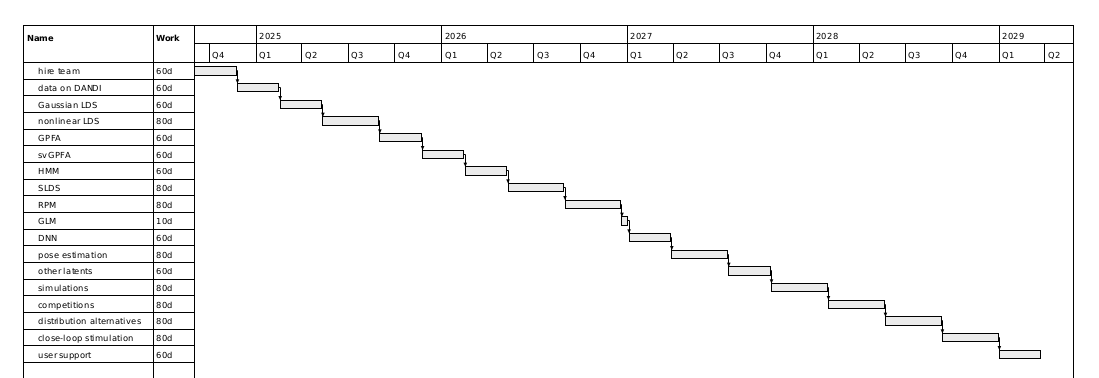
\includegraphics[width=5in]{figures/bbr24TasksCropped.png}

    \caption{Schedule of proposed tasks. Note that it is difficult to forecast
    the exact trajectory of the project, as unexpected challenges may appear in
    the development of methods to process a radically new type of data.}

    \label{fig:gnattChart}
\end{figure}
% \item[visualization of very large experimental data]
% \item[data compression]
% \item[close loop foraging experimentation]

